%%%%%% CMB-S4 Simulations and Data Analysis Chapter  %%%%%%%%%%%%%%%%
 
\chapter{Simulations and Data Analysis}
\renewcommand*\thesection{\arabic{section}}

%%%%%%%%%%%%%%%%%%%%%%%%%%%%%%%%%%%%%%%%%%%%%%%%%%%%%%%%%%%
%%%%%%%%%%%%%%%%%%%%%%%%%%%%%%%%%%%%%%%%%%%%%%%%%%%%%%%%%%%
%%%%%%%%%%%%%%%%%%%%%%%%%%%%%%%%%%%%%%%%%%%%%%%%%%%%%%%%%%%
%%%%%%%%%%%%%%%%%%%%%%%%%%%%%%%%%%%%%%%%%%%%%%%%%%%%%%%%%%%

\section{Introduction}

Extracting science from a CMB dataset is a complex, iterative process requiring expertise in both physical and computational sciences. In this chapter we start by outlining the data analysis pipeline and describing how this is complicated by various real-world issues ranging from instrument systematics to computational tractability. We then discuss the drivers for, and corresponding structure of, the simulation pipeline. Next we couple these into an overall simulation and data analysis pipeline, and motivate the division of this pipeline into 5 subsets based on the challenges they pose and the expertise required to meet these. Finally we consider each of these subsets in turn, sketching their current state of the art and noting the prospects for addressing their challenges in the context of the CMB-S4 mission.

\subsection{Data Analysis}

The reduction of a CMB data set typically proceeds in a sequence of steps:
\begin{figure}[htbp]
\begin{minipage}[h]{0.7\linewidth}
\begin{description}
\item[ Pre-processing:] The raw time-ordered detector data are calibrated and gross time-domain systematics are either removed (typically by template subtraction or filtering) or flagged. The goal here is to make the real data match a model that will underpin all subsequent analyses.
\item[Map-making:] At each observing frequency, estimates of the intensity I and the Stokes Q- and U-polarizations of the sky signal are extracted from the cleaned time-ordered data based on their spatial stationarity, typically using some degree of knowledge of the instrument's noise properties.
\item[Component separation:] The CMB is separated from the various foreground sky components using the set of frequency maps and relying on its unique spectral invariance (in CMB units).
\item[Power spectrum estimation:] The six auto- and cross-angular power spectra of the CMB intensity and E- and B-mode polarizations are estimated from the autocorrelation of the CMB maps or the cross-correlation of the frequency maps, and corrected for E- to B-mode lensing.
\item[Parameter estimation:] The best-fit parameters for any cosmological model are derived by comparing the theoretical CMB power spectra that they would induce with the data and their uncertainties.
\end{description}
\end{minipage}
\begin{minipage}[h]{0.3\linewidth}
\centering
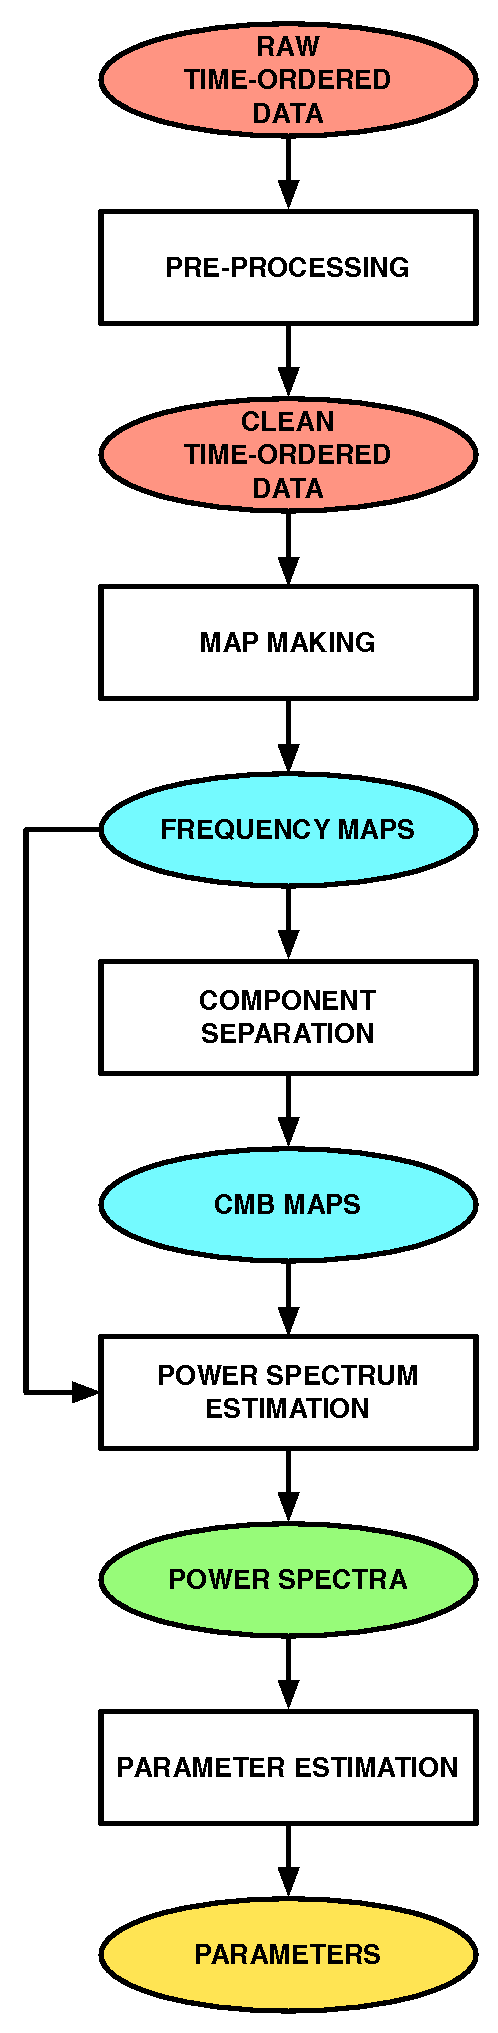
\includegraphics[width=0.45\textwidth]{Analysis/dr}
\end{minipage}
\end{figure}

This reduction essentially consists of a series of changes of basis for the data, from time samples (red) to map pixels (blue) to spectral multipoles (green) to cosmological parameters (yellow), with each basis-change reducing the data volume, increasing the signal-to-noise, and exposing a different class of systematic effects for mitigation.

Note however that the data can only remain a sufficient statistic at each step in the reduction if we also propagate its full covariance matrix. Since this is an ${\cal N}_b \times {\cal N}_b$ matrix in the dimension of the basis, its construction, manipulation and reduction pose the greatest computational challenge to this analysis. In particular, except in special cases the full pixel-domain data covariance matrix is dense and unstructured, requiring O(${\cal N}_p^3$) operations to build and O(${\cal N}_p^2$) bytes to store. All the major drivers of CMB science - polarization sensitivity, higher resolution, larger sky coverage - push us towards larger pixel counts, with an instrument mapping a fraction of the sky $f_{sky}$ with a beam of $b$ arcminutes covering O($10^9 \, f_{sky}/b^2$) pixels per IQU-component. For the last decade or more the computational intractability of the resulting pixel-domain matrices has forced us to replace explicit covariance propagation with Monte Carlo methods in all but a limited set of small sky fraction/low resolution cases.

\begin{figure}[htbp]
\centering
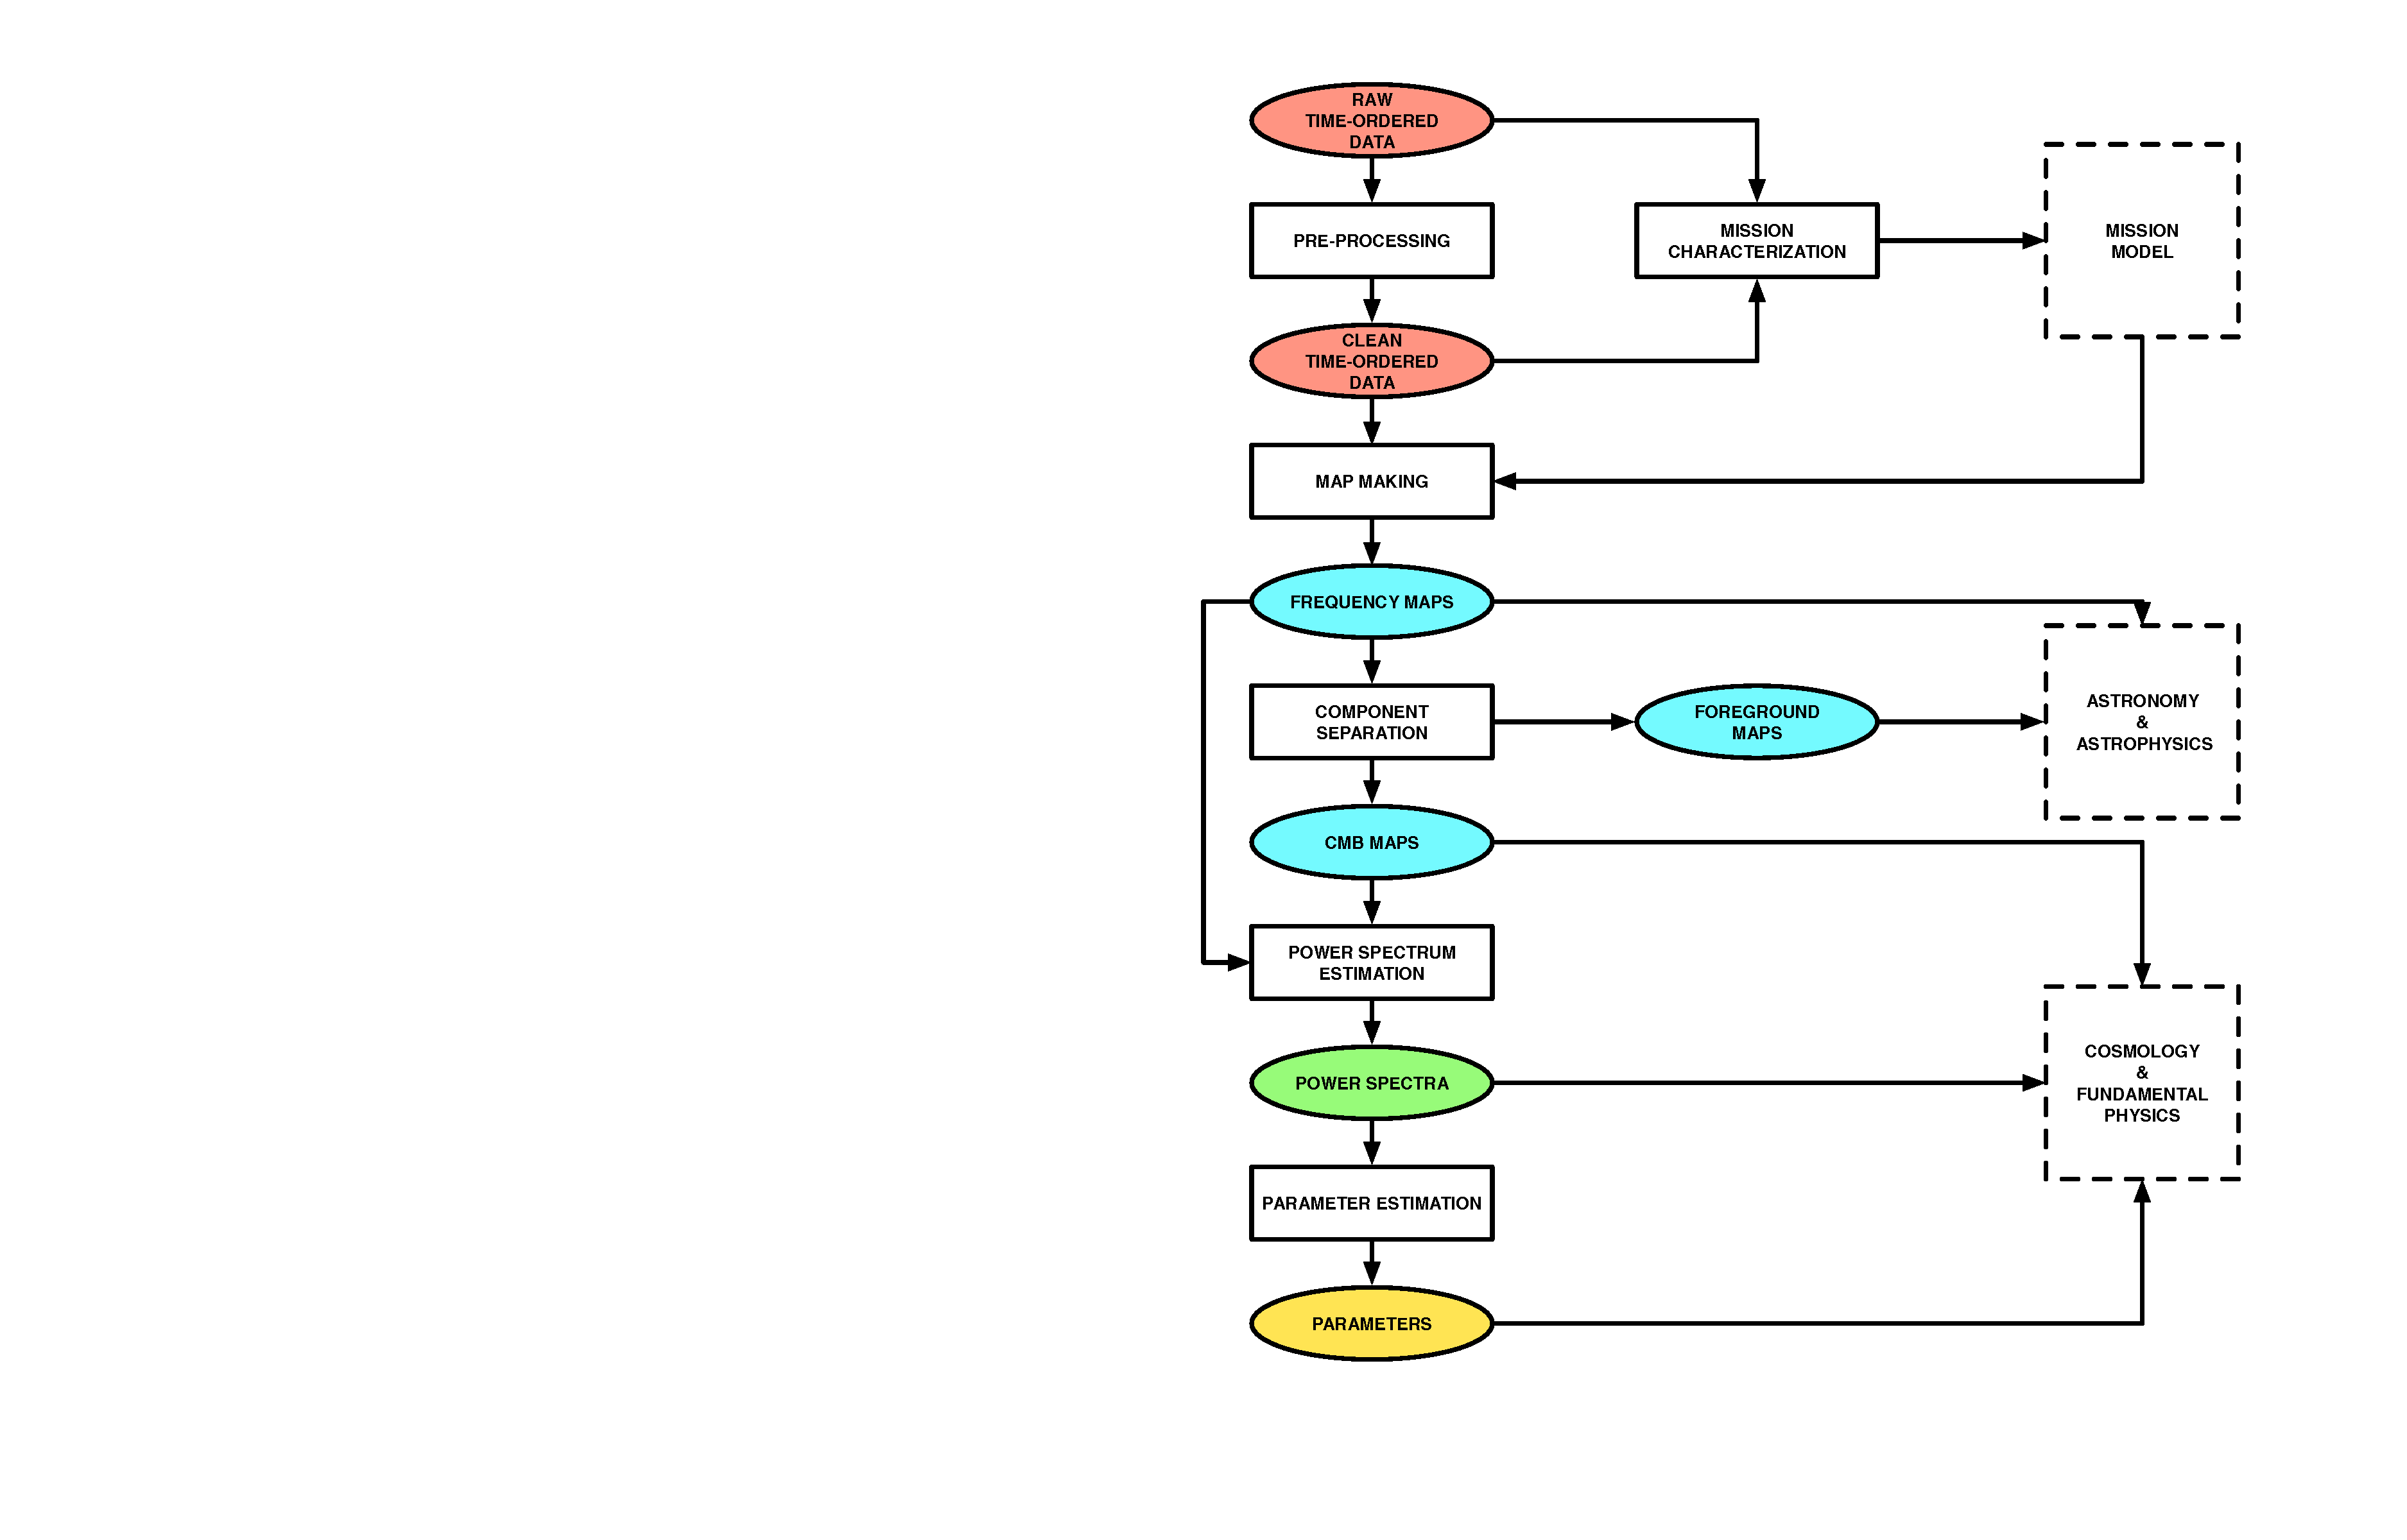
\includegraphics[width=0.575\textwidth]{Analysis/da}
\caption{The CMB data analysis pipeline}
\label{fig_da}
\end{figure}

Beyond this basic data reduction, the full analysis pipeline (Figure \ref{fig_da}) also includes mission characterization and science exploitation branches. For the former, the time-ordered data are extensively used to build a model of the mission itself, comprising both the instrument and the observation. This can include such processes as determining beam properties from planet crossings; estimating noise properties (including cross-correlations) from calibrated, signal-subtracted, time-ordered data; and reconstructing the telescope pointing solution from ancilliary time-domain data such as star-trackers. The resulting mission model then feeds back into all of the ensuing data reduction and interpretation. For the latter, given sufficient observing frequencies we can not simply perform foreground removal, but rather component separation, where the individual foreground components are isolated based on their different (possibly spatially varying) spectral dependencies; such component maps then provide important inputs to astronomy and astrophysics. Similarly a wide range of analyses of the CMB maps, power spectra and parameters collectively inform our understanding of cosmology and fundamental physics, including measurements of the energy scale of inflation and the sum of neutrino masses from the power spectra and of cosmological non-Gaussianity from the higher-order statistics of the CMB maps.

\subsection{Simulation}

Simulations of a CMB mission's data play a number of critical roles; specifically they are required for
\begin{itemize}
\item The design and development of both the instrument and the observation, to ensure that the mission is capable of meeting its science goals.
\item The validation and verification of all data analysis tools, including those used in data reduction, mission charaterization and science explopitation.
\item Monte Carlo based uncertainty quantification and debiasing, particularly when the full data covariance matrix is computationally intractable.
\end{itemize}

As shown in Figure \ref{fig_sim}, given a mission model (both instrument and observation) and a sky model (both CMB and foregrounds) we can generate a simulation of the mission data in any of its domains. However, there is an inevitable trade-off between how representative the simulation is of real data and the complexity of the input models and computational cost of generating the simulation. The choice of the simulation data domain will then be determined by the balance between the realism requirements and the complexity/cost constraints for the particular task at hand.

\begin{figure}[htbp]
\centering
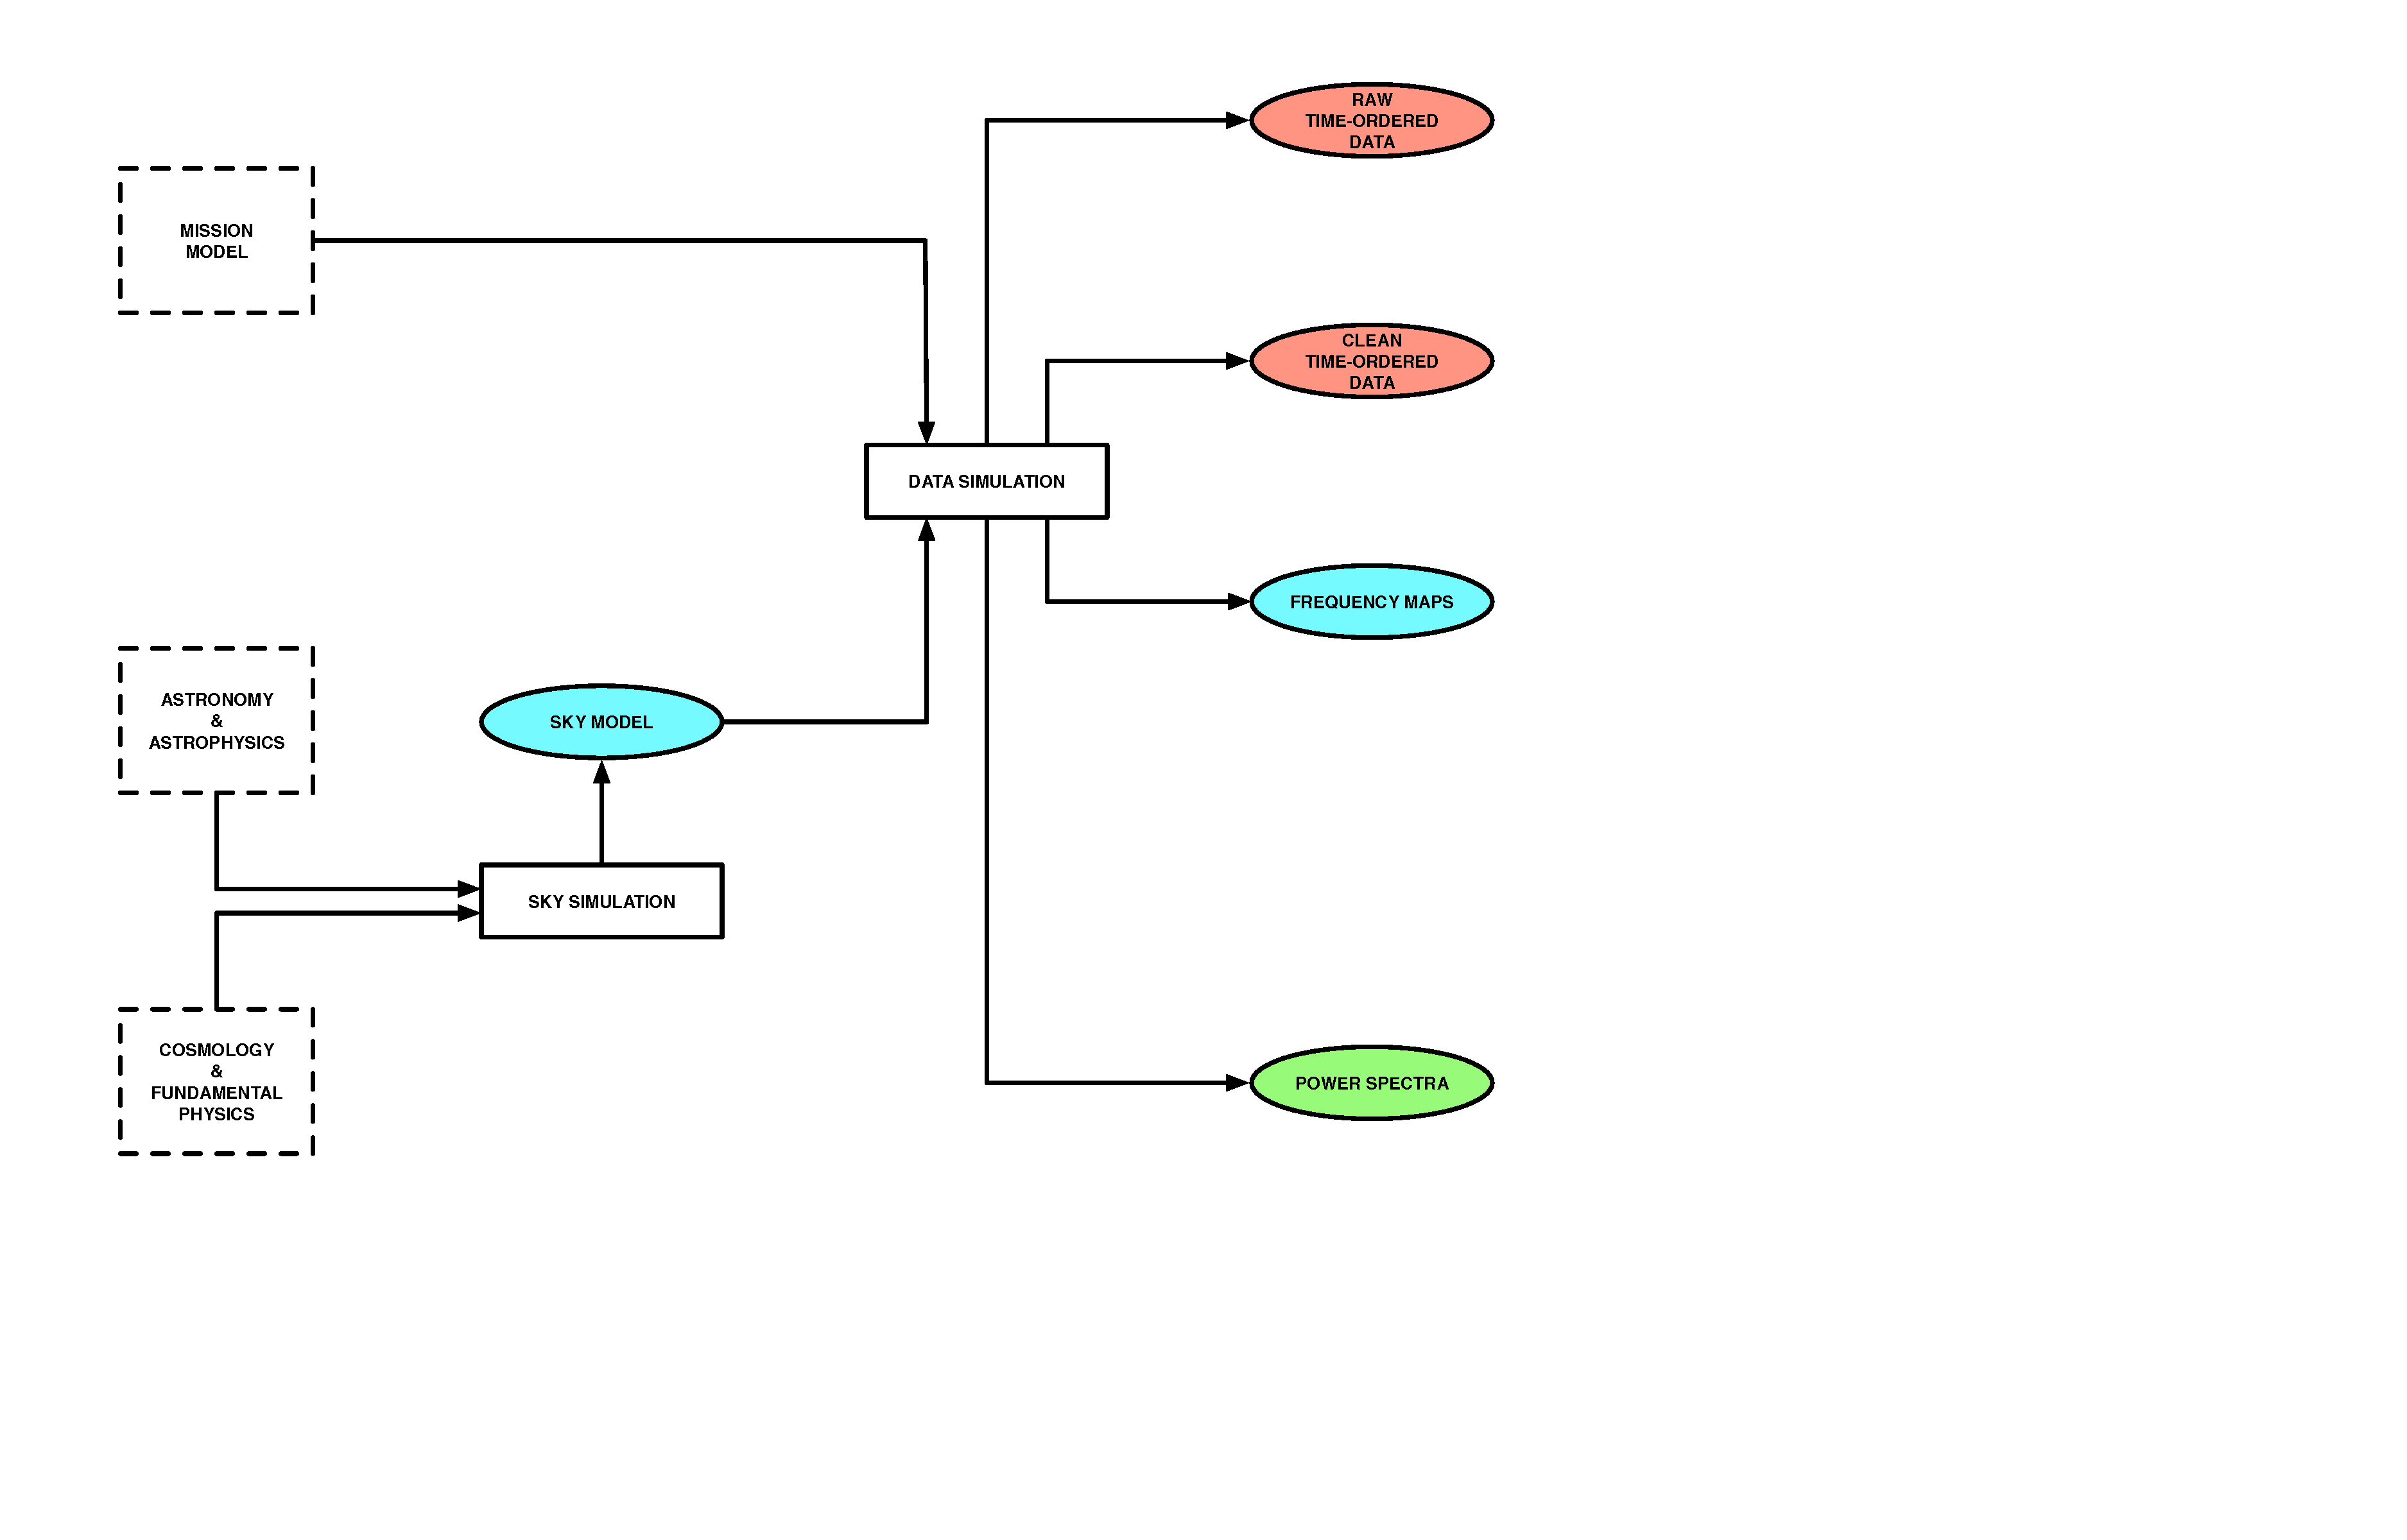
\includegraphics[width=0.575\textwidth]{Analysis/sim}
\caption{The CMB simulation pipeline}
\label{fig_sim}
\end{figure}

Note that the generation of the input mission and sky models are themselves far from trivial tasks. The mission model is typically derived from pre-deployment measurements of the instrument properties refined by characterization from the data themselves, together with ancilliary pointing and environmental data characterizing the observation; the sky model requires its own dedicated simulation capability which - since it is independet of the details of any single mission - can be a community-side endeavor common to many.

\subsection{Simulation and Data Analysis}

Coupling the above, the overall simulation and data analysis pipeline (Figure \ref{fig_simda}) can now be seen as both as a top-down data reduction process and a right-to-left refinement of our mission and sky modeling. Typically we alternate between the two phases, with each new data reduction improving our mission and sky models, which models are in turn are fed back into an improved data reduction.

\begin{figure}[htbp]
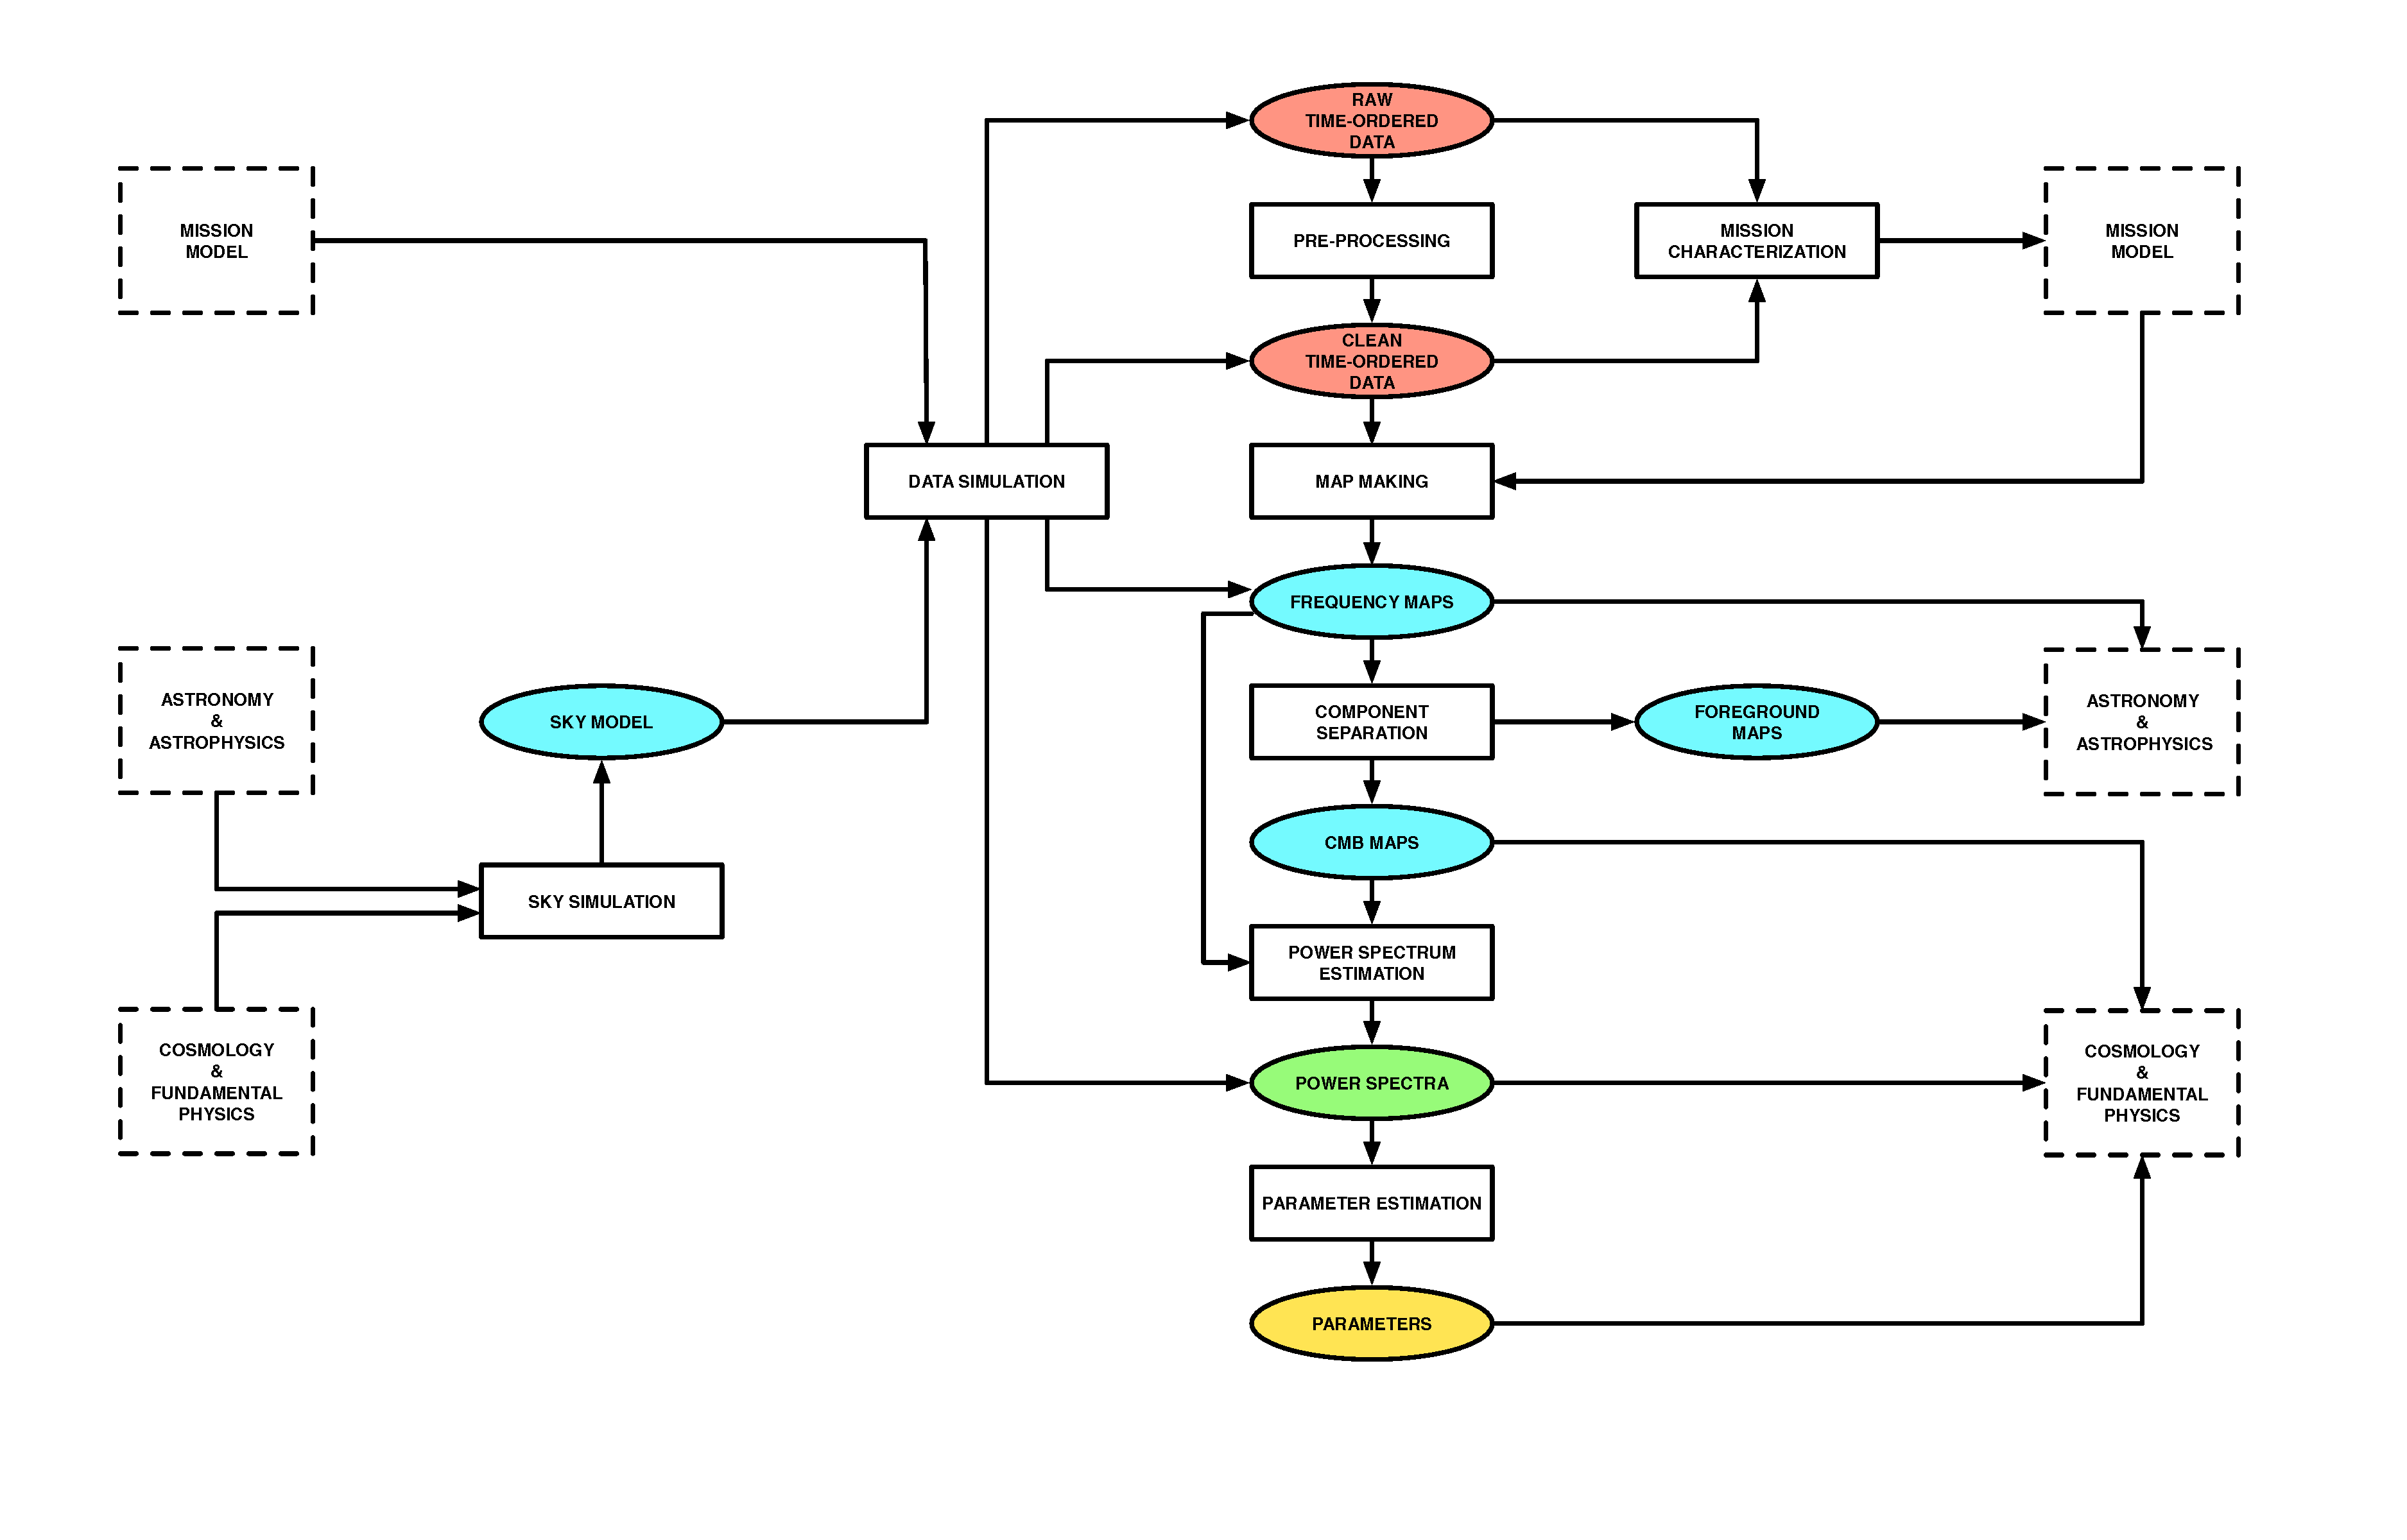
\includegraphics[width=1\textwidth]{Analysis/simda}
\caption{The full CMB simulation and data analysis pipeline}
\label{fig_simda}
\end{figure}

The implementation and execution of this pipeline still poses many challenges to the CMB community, and we can subdivide it into 5 subsets based on the nature of the challenges posed and the expertise and activity required to address them:
\begin{description}
\item[Forecasting:] The rapid assessment of nominal scientific performance under sufficiently simplifying mission and sky models that all analysis can be done in the spectral domain.
\item[Sky modeling:] Mission-independent modeling of the CMB (scalar, tensor and non-Gausian) and the astrophysical foregrounds, including the couplings between them.
\item[Time-ordered data processing:] All processes that require the manipulation of time-domain data, dominated by the associated `Big Data' challenges.
\item[Component separation:] Separation of the CMB from the foreground sky, and ideally separation of the individual foreground components to feed back into sky modeling.
\item[Statistics and parameters:] Derivation of the CMB statistics, including 2-, 3-, and 4-point correlation functions, together with the parameters of cosmology and fundamental physics that they constrain.
\end{description}

\newpage

\input Analysis/forecasting.tex

\newpage

\input Analysis/sky_modeling.tex

\newpage

\input Analysis/tod_processing.tex

\newpage

\input Analysis/component_separation.tex

\newpage

\input Analysis/statistics_parameters.tex

\newpage

%\bibliography{cmbs4}

%%
%% Populate the .bib file with entries from SPIRES Bibtex (preferred)
%% or ADS Bibtex (if no SPIRES entry).
%%  SPIRES will also supply the CITATION line information; please include it.
%%


